\documentclass{article}
\usepackage{algorithmic}
\usepackage{graphicx}
\usepackage{amsmath}
\usepackage{natbib}
\usepackage[linesnumbered,ruled,vlined]{algorithm2e}
\title{Algoritmos y Estructuras de Datos III \\ Trabajo Pr\'{a}ctico 1}
\author{Mart\'{i}n Arjovsky 683/12\\ Ezequiel Dar\'io Gambaccini \\ Silvio Vileri\~no}
\date{Abril 2014}

\begin{document}
 \maketitle
  
  \section{Ejercicio 2}
  
  A continuaci\'on se muestran los gr\'aficos del lote 2 para 1, 2 y 3 n\'ucleos.
  \begin{figure}[htb]
  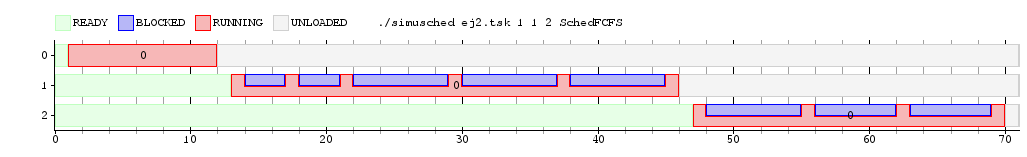
\includegraphics[scale=0.32]{ej2_1.png}
  \caption{Diagrama de Gantt para el lote 2 en FCFS con un n\'ucleo}
  \end{figure}
  \begin{figure}[htb]
  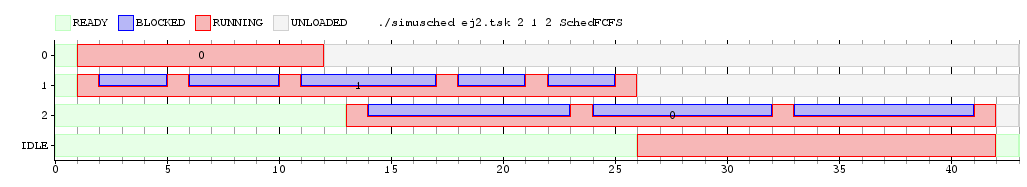
\includegraphics[scale=0.32]{ej2_2.png}
  \caption{Diagrama de Gantt para el lote 2 en FCFS con dos n\'ucleos}
  \end{figure}
  \begin{figure}[htb]
  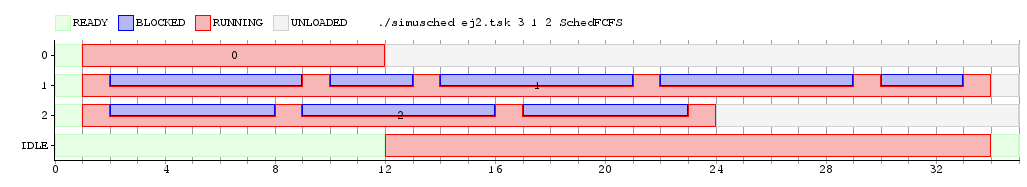
\includegraphics[scale=0.32]{ej2_3.png}
  \caption{Diagrama de Gantt para el lote 2 en FCFS con tres n\'ucleos}
  \end{figure}
 
  \section{Ejercicio 4}
  
  A continuaci\'on se muestran los gr\'aficos del lote 4 ejecutado en el scheduler Round-Robin.
  \begin{figure}[htb]
  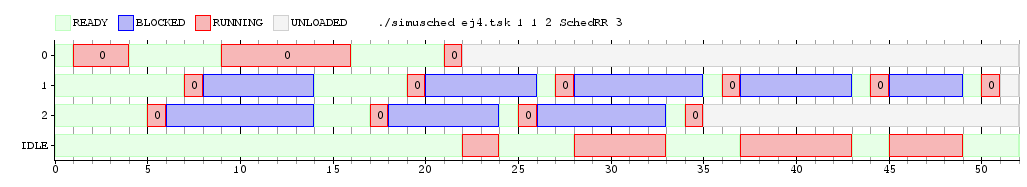
\includegraphics[scale=0.32]{ej4_1.png}
  \caption{Diagrama de Gantt para el lote 4 en RR con un n\'ucleo}
  \end{figure}
  \begin{figure}[htb]
  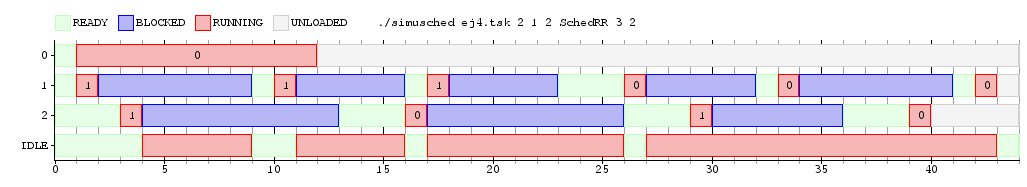
\includegraphics[scale=0.32]{ej4_2.png}
  \caption{Diagrama de Gantt para el lote 4 en RR con dos n\'ucleos}
  \end{figure}
  
  En ambos gr\'aficos se observa el comportamiento esperado de un scheduler de tipo Round-Robin. En particular, en la figura 4 se ve como la tarea 0 corre en el \'unico n\'ucleo hasta que en el tiempo 4 se le acaba
  el quantum disponible y el scheduler busca otro proceso disponible en la cola global. Tambi\'en se muestra repetidamente como cuando un proceso realiza una llamada bloqueante, el CPU deja esa tarea para ir a ejecutar
  otra. En la figura 5 se observa el mismo comportamiento, pero adem\'as podemos observar la migraci\'on de procesos entre n\'ucleos, por ejemplo a tiempo 16 en la tarea 2.
  
  \section{Ejercicio 7}
  
  Para estudiar la performance del Round-Robin variando los cuantos creamos el lote7 y realizamos varias simulaciones. Variamos los quantums entre 1 y 10 inclusive y evaluamos el throughput y INSERTAR SEGUNDA M\'ETRICA con 2 y 4 n\'ucleos. Como las tareas TaskConsola son pseudoaleatorias,
  para cada seleccio\'on de par\'ametros corrimos 10 simulaciones y graficamos el promedio con la variaci\'on estandard.
  
  \begin{figure}
  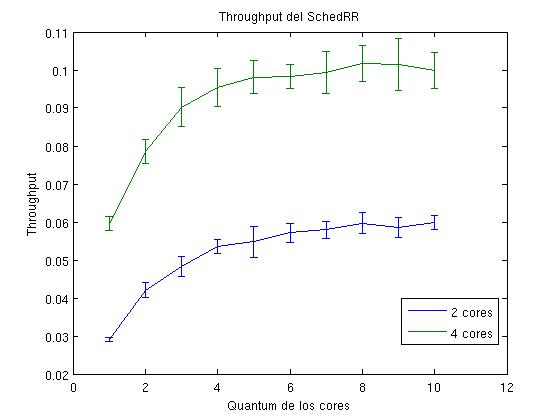
\includegraphics[scale=0.6]{TH.jpg}
  \caption{Throughput para SchedRR con dos y cuatro n\'ucleos}
  \end{figure}
  
  En la figura 6 se muestran los resultados del throughput. En la misma se observa que (considerando las desviaciones) el throughput aumenta al aumentar el quantum, tanto para 2 como 4 n\'ucleos. Esto tiene mucho sentido, ya que se
  gasta menos tiempo en cambios de contexto y es menos probable que un proceso cambie de CPU, bajando el costo total de migraci\'on de procesos entre CPUs. Obviamente, este crecimiento converge, ya que el tiempo que tardan en terminar los procesos est\'a acotado por
  el uso total del CPU dividido la cantidad de n\'ucleos, por lo que el throughput tambi\'en converge.
  
  \section{Ejercicio 8}
  
  A continuaci\'on se muestran los gr\'aficos del lote 8 ejecutado sobre los schedulers Round-Robin con y sin migraci\'on entre procesos.
  
  \begin{figure}
  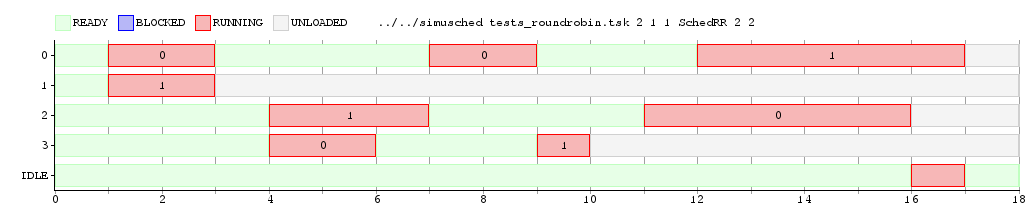
\includegraphics[scale=0.32]{ej8_RR.png}
  \caption{Diagrama de Gantt para el lote 8 en RR con dos n\'ucleos}
  \end{figure}
  
  \begin{figure}
  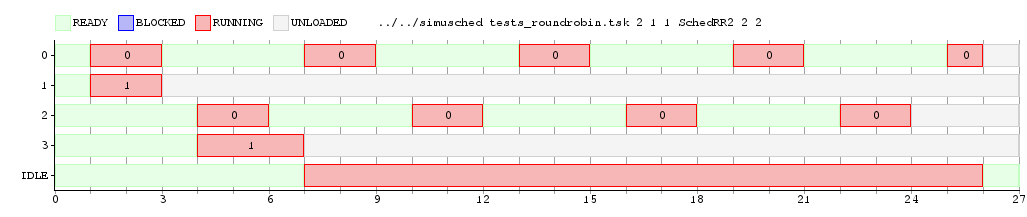
\includegraphics[scale=0.32]{ej8_RR2.png}
  \caption{Diagrama de Gantt para el lote 8 en RR2 con dos n\'ucleos}
  \end{figure}
 
  Se puede observar en el caso donde hay tareas con considerable diferencia de duracion, una mejor performance del scheduler RR1, dado que realiza una correccion permanente del balanceo de carga usando los recursos que tiene a su alcance en cada tick. Mientras que en el RR2, al quedar fija la afinidad al momento del dispatch, si ocurre un caso donde ambas tareas cortas quedan en un core y las tareas largas en otro core, al finalizar las tareas cortas, se desperdiciara un core durante toda la ejecucion de las tareas largas.
  Esta diferencia se ve claramente en los gr\'aficos 7 y 8 si notamos que cuando se usa RR1 se termina de ejecutar a tiempo 18 y con RR2 a tiempo 27, lo que es una diferencia abismal. Cabe destacar que para que esto pase se necesita
  que haya una gran diferencia entre el uso de CPU de las tareas y que las largas se encuentren concentradas en un n\'ucleo mientras las cortas en otro, lo que no suele ser un caso promedio.
\end{document}
